\documentclass{article}

\usepackage[bottom=1cm, right=1cm, left=1cm, top=1cm]{geometry}
\pagenumbering{gobble}

\usepackage{multirow}
\usepackage{makecell}

\usepackage{musixtex}
\usepackage{guitarchordschemes}
\usepackage{tikz}

\def\musicintext#1{
  {\let\extractline\relax
   \nobarnumbers
   \staffbotmarg0pt
   \startextract\addspace{-\afterruleskip}\qsk#1\endextract}}

\setchordscheme{
    rotate = -90,
    tuning = {,,,,,},
    restrict-bounding-box = true,
    x-unit=1.75mm,
    y-unit=2.75mm,
    line-width = 0.4pt,
    finger-radius = .5,
    % position = {<tex code>},
    % ringing-style = {draw, fill = red},
    muted-style = {cross out, draw, scale = 0.65}
}

\begin{document}

{
\centering
\begin{tabular}{ p{2.9cm} p{1cm} p{3.15cm} p{1.75cm} p{4.25cm} p{1.6cm} p{1.9cm} }
    \multicolumn{7}{c}{\Huge{Jazz Chords in C}} \\
    \hline
        \makecell[cl]{
            \textcolor{blue}{Minor Seventh}} &
        \makecell[cl]{
            Cmin\textsuperscript{7} \\
            Cm\textsuperscript{7} \\
            C\textminus\textsuperscript{7}} &
        \makecell[cl]{
            Minor Seventh \\
            Minor Triad} &
        \makecell[cc]{
            \raisebox{0ex}[5ex][1ex]{
                \musicintext{\staffbotmarg2\Interligne
                \Notes \zw{c}\accshift=0.6mm\zw{_e}\accshift=0mm\zw{g}\zw{_i}\en}}} &
        \makecell[cc]{
            \begin{tikzpicture}
                \node{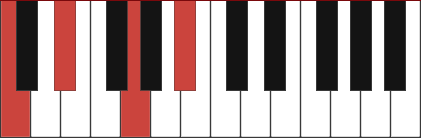
\includegraphics[width=0.2\textwidth]{assets/cm7.png}};
            \end{tikzpicture}} &
        \makecell[cc]{
            \chordscheme[
                position = 3,
                barre = 1/1-5,
                finger = 2/2,
                finger = 3/4,
                mute = 6
            ]} & \\
    \hline
        \makecell[cl]{
            \textcolor{red}{Dominant Seventh}} &
        \makecell[cl]{
            C\textsuperscript{7}} &
        \makecell[cl]{
            Minor Seventh \\
            Major Triad} &
        \makecell[cc]{
            \raisebox{0ex}[5ex][1ex]{
                \musicintext{\staffbotmarg2\Interligne
                \Notes \zw{c}\zw{e}\zw{g}\zw{_i}\en}}} &
        \makecell[cc]{
            \begin{tikzpicture}
                \node{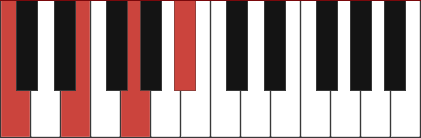
\includegraphics[width=0.2\textwidth]{assets/c7.png}};
            \end{tikzpicture}} &
            \makecell[cc]{
                \chordscheme[
                    finger = 1/2,
                    finger = 3/3,
                    finger = 2/4,
                    finger = 3/5,
                    mute = 6,
                    ring = 1
                ]} &
        \makecell[cl]{
            \footnotesize{C\textsuperscript{7$\flat$5}: dim 5\textsuperscript{th}} \\
            \footnotesize{C\textsuperscript{7\textminus5}: dim 5\textsuperscript{th}} \\
            \footnotesize{C\textsuperscript{7$\sharp$5}: aug 5\textsuperscript{th}} \\
            \footnotesize{C\textsuperscript{7+5}: aug 5\textsuperscript{th}} \\
        } \\
    \hline
        \makecell[cl]{
            \textcolor[RGB]{0,150,20}{Major Seventh}} &
        \makecell[cl]{
            Cmaj\textsuperscript{7} \\
            CM\textsuperscript{7} \\
            C$\Delta$\textsuperscript{7}} &
        \makecell[cl]{
            Major Seventh \\
            Major Triad} &
        \makecell[cc]{
            \raisebox{0ex}[5ex][1ex]{
                \musicintext{\staffbotmarg2\Interligne
                \Notes \zw{c}\zw{e}\zw{g}\zw{i}\en}}} &
        \makecell[cc]{
            \begin{tikzpicture}
                \node{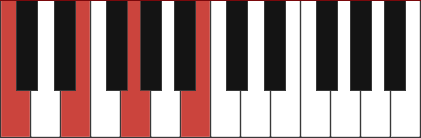
\includegraphics[width=0.2\textwidth]{assets/cmaj7.png}};
            \end{tikzpicture}} &
        \makecell[cc]{
            \chordscheme[
                finger = 2/4,
                finger = 3/5,
                mute = 6,
                ring = {1,2,3}
            ]} & \\
    \hline
        \makecell[cl]{
            Major Sixth} &
        \makecell[cl]{
            C\textsuperscript{6}} &
        \makecell[cl]{
            Major Sixth \\
            Major Triad} &
        \makecell[cc]{
            \raisebox{0ex}[5ex][1ex]{
                \musicintext{\staffbotmarg2\Interligne
                \Notes \zw{c}\zw{e}\zw{g}\qsk\zw{h}\en}}} &
        \makecell[cc]{
            \begin{tikzpicture}
                \node{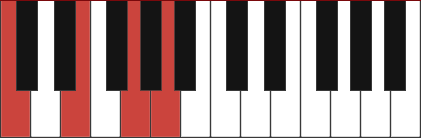
\includegraphics[width=0.2\textwidth]{assets/c6.png}};
            \end{tikzpicture}} &
        \makecell[cc]{
            \chordscheme[
                finger = 1/2,
                finger = 2/3,
                finger = 2/4,
                finger = 3/5,
                mute = 6,
                ring = 1
            ]} &
        \makecell[cl]{
            \footnotesize{Cm\textsuperscript{6}: dim 3\textsuperscript{rd}} \\
            \footnotesize{C\textsuperscript{6/9}: add 9\textsuperscript{th}}
        } \\
    \hline
        \makecell[cl]{
            \textcolor{orange}{Diminished}} &
        \makecell[cl]{
            C\textsuperscript{o} \\
            Cdim} &
        \makecell[cl]{
            Diminished Fifth \\
            Minor Third \\
            Root} &
        \makecell[cc]{
            \raisebox{0ex}[5ex][1ex]{
                \musicintext{\staffbotmarg2\Interligne
                \Notes \hqsk\zw{c}\accshift=1.4mm\zw{_e}\accshift=0mm\zw{_g}\en}}} &
        \makecell[cc]{
            \begin{tikzpicture}
                \node{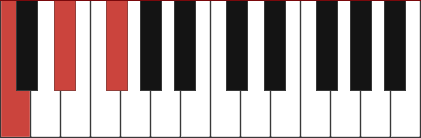
\includegraphics[width=0.2\textwidth]{assets/cdim.png}};
            \end{tikzpicture}} &
        \makecell[cc]{
            \chordscheme[
                position = 3,
                finger = 2/2,
                finger = 3/3,
                finger = 2/4,
                finger = 1/5,
                mute = {1,6}
            ]} &
        \makecell[cl]{
            \footnotesize{interchangable} \\
            \footnotesize{with C\textsuperscript{o7}}
        } \\
    \hline
        \makecell[cl]{
            Fully Diminished \\
            Seventh} &
        \makecell[cl]{
            C\textsuperscript{o7} \\
            Cdim\textsuperscript{7}} &
        \makecell[cl]{
            Diminished Seventh \\
            \textcolor{orange}{Diminished}} &
        \makecell[cc]{
            \raisebox{0ex}[5ex][1ex]{
                \musicintext{\staffbotmarg2\Interligne
                \Notes \qsk\zw{c}\accshift=0.4mm\zw{_e}\accshift=2.8mm\zw{_g}\accshift=0mm\zw{<i}\en}}} &
        \makecell[cc]{
            \begin{tikzpicture}
                \node{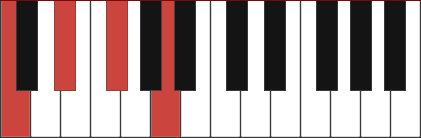
\includegraphics[width=0.2\textwidth]{assets/cdim7.png}};
            \end{tikzpicture}} &
        \makecell[cc]{
            \chordscheme[
                position = 7,
                finger = 2/3,
                finger = 1/4,
                finger = 3/5,
                finger = 2/6,
                mute = {1,2},
            ]} &
        \makecell[cl]{
            \footnotesize{interchangable} \\
            \footnotesize{with C\textsuperscript{o}}
        } \\
    \hline
        \makecell[cl]{
            Half Diminished \\
            Seventh} &
        \makecell[cl]{
            C\textsuperscript{\o{}7} \\
            Cm\textsuperscript{7$\flat$5} \\
            C\textminus\textsuperscript{7$\flat$5}} &
        \makecell[cl]{
            Minor Seventh \\
            \textcolor{orange}{Diminished}} &
        \makecell[cc]{
            \raisebox{0ex}[5ex][1ex]{
                \musicintext{\staffbotmarg2\Interligne
                \Notes \tqsk\zw{c}\accshift=0.4mm\zw{_e}\accshift=2.2mm\zw{_g}\accshift=0mm\zw{_i}\en}}} &
        \makecell[cc]{
            \begin{tikzpicture}
                \node{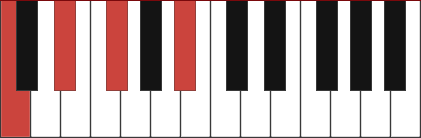
\includegraphics[width=0.2\textwidth]{assets/cm7b5.png}};
            \end{tikzpicture}} &
        \makecell[cc]{
            \chordscheme[
                position = 3,
                barre = 1/3-5,
                finger = 4/1,
                finger = 2/2,
                finger = 2/4,
                mute = 6
            ]} &
        \makecell[cl]{
            \footnotesize{can also be} \\
            \footnotesize{thought of as} \\
            \footnotesize{Cm\textsuperscript{7} with a} \\
            \footnotesize{dim 5\textsuperscript{th}}
        } \\
    \hline
        \makecell[cl]{
            Minor Ninth} &
        \makecell[cl]{
            Cm\textsuperscript{9}} &
        \makecell[cl]{
            Major Ninth \\
            \textcolor{blue}{Minor Seventh}} &
        \makecell[cc]{
            \raisebox{0ex}[5ex][1ex]{
                \musicintext{\staffbotmarg2\Interligne
                \Notes \zw{c}\accshift=0.6mm\zw{_e}\accshift=0mm\zw{g}\zw{_i}\zw{k}\en}}} &
        \makecell[cc]{
            \begin{tikzpicture}
                \node{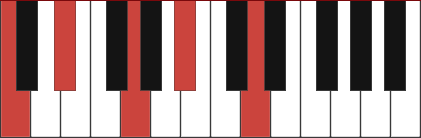
\includegraphics[width=0.2\textwidth]{assets/cm9.png}};
            \end{tikzpicture}} &
        \makecell[cc]{
            \chordscheme[
                position = 6,
                finger = 2/3,
                finger = 3/4,
                finger = 1/5,
                finger = 3/6,
                mute = {1,2}
            ]} & \\
    \hline
        \makecell[cl]{
            \textcolor[RGB]{80,0,150}{Dominant Ninth}} &
        \makecell[cl]{
            C\textsuperscript{9}} &
        \makecell[cl]{
            Major Ninth \\
            \textcolor{red}{Dominant Seventh}} &
        \makecell[cc]{
            \raisebox{0ex}[5ex][1ex]{
                \musicintext{\staffbotmarg2\Interligne
                \Notes \zw{c}\zw{e}\zw{g}\zw{_i}\zw{k}\en}}} &
        \makecell[cc]{
            \begin{tikzpicture}
                \node{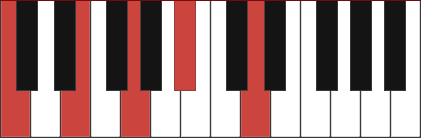
\includegraphics[width=0.2\textwidth]{assets/c9.png}};
            \end{tikzpicture}} &
        \makecell[cc]{
            \chordscheme[
                finger = 3/2,
                finger = 3/3,
                finger = 2/4,
                finger = 3/5,
                mute = 6,
                ring = 1
            ]} &
        \makecell[cl]{
            \footnotesize{opt. 5\textsuperscript{th}}
        } \\
    \hline
        \makecell[cl]{
            Major Ninth} &
        \makecell[cl]{
            Cmaj\textsuperscript{9}} &
        \makecell[cl]{
            Major Ninth \\
            \textcolor[RGB]{0,150,20}{Major Seventh}} &
        \makecell[cc]{
            \raisebox{0ex}[5ex][1ex]{
                \musicintext{\staffbotmarg2\Interligne
                \Notes \zw{c}\zw{e}\zw{g}\zw{i}\zw{k}\en}}} &
        \makecell[cc]{
            \begin{tikzpicture}
                \node{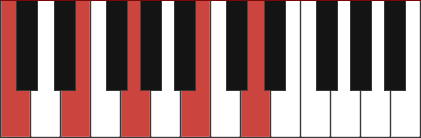
\includegraphics[width=0.2\textwidth]{assets/cmaj9.png}};
            \end{tikzpicture}} &
        \makecell[cc]{
            \chordscheme[
                finger = 3/2,
                finger = 4/3,
                finger = 2/4,
                finger = 3/5,
                mute = {1,6}
            ]} & \\
    \hline
        \makecell[cl]{
            Eleventh} &
        \makecell[cl]{
            C\textsuperscript{11}} &
        \makecell[cl]{
            Perfect Eleventh \\
            \textcolor[RGB]{80,0,150}{Dominant Ninth}} &
        \makecell[cc]{
            \raisebox{0ex}[5ex][1ex]{
                \musicintext{\staffbotmarg2\Interligne
                \Notes \zw{c}\zw{g}\zw{_i}\zw{k}\zw{m}\en}}} &
        \makecell[cc]{
            \begin{tikzpicture}
                \node{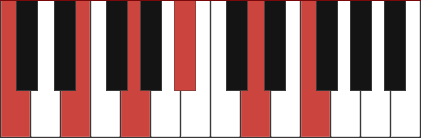
\includegraphics[width=0.2\textwidth]{assets/c11.png}};
            \end{tikzpicture}} &
        \makecell[cc]{
            \chordscheme[
                barre = 3/1-5,
                mute = 6
            ]} &
        \makecell[cl]{
            \footnotesize{omit 3\textsuperscript{rd}} \\
            \footnotesize{opt. 1\textsuperscript{st}} \\
            \footnotesize{opt. 5\textsuperscript{th}} \\
            \footnotesize{opt. 9\textsuperscript{th}}
        } \\
    \hline
        \makecell[cl]{
            Thirteenth} &
        \makecell[cl]{
            C\textsuperscript{13}} &
        \makecell[cl]{
            Major Thirteenth \\
            \textcolor[RGB]{80,0,150}{Dominant Ninth}} &
        \makecell[cc]{
            \raisebox{0ex}[5ex][1ex]{
                \musicintext{\staffbotmarg2\Interligne
                \Notes \zw{c}\zw{e}\zw{g}\zw{_i}\zw{k}\zw{o}\en}}} &
        \makecell[cc]{
            \begin{tikzpicture}
                \node{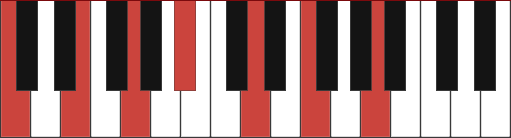
\includegraphics[width=0.2\textwidth]{assets/c13.png}};
            \end{tikzpicture}} &
        \makecell[cc]{
            \chordscheme[
                position = 8,
                finger = 3/2,
                finger = 2/3,
                finger = 1/4,
                finger = 1/6,
                mute = {1,5}
            ]} &
        \makecell[cl]{
            \footnotesize{opt. 1\textsuperscript{st}} \\
            \footnotesize{opt. 5\textsuperscript{th}} \\
            \footnotesize{opt. 9\textsuperscript{th}}
        } \\
    \hline
        \makecell[cl]{
            Augmented} &
        \makecell[cl]{
            C\textsuperscript{+} \\
            Caug \\
            C\textsuperscript{$\sharp$5}} &
        \makecell[cl]{
            Augmented Fifth \\
            Major Third \\
            Root} &
        \makecell[cc]{
            \raisebox{0ex}[5ex][1ex]{
                \musicintext{\staffbotmarg2\Interligne
                \Notes \zw{c}\zw{e}\zw{^g}\en}}} &
        \makecell[cc]{
            \begin{tikzpicture}
                \node{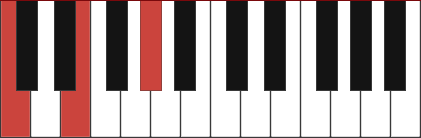
\includegraphics[width=0.2\textwidth]{assets/caug.png}};
            \end{tikzpicture}} &
        \makecell[cc]{
            \chordscheme[
                finger = 1/2,
                finger = 1/3,
                finger = 2/4,
                finger = 3/5,
                mute = 6,
                ring = 1
            ]} &
        \makecell[cl]{
            \footnotesize{Caug\textsuperscript{7} is} \\
            \footnotesize{identical to} \\
            \footnotesize{C\textsuperscript{7+5}}
        } \\
    \hline
    \makecell[cl]{
            Suspended} &
        \makecell[cl]{
            Csus2} &
        \makecell[cl]{
            Perfect Fifth \\
            Major Second \\
            Root} &
        \makecell[cc]{
            \raisebox{0ex}[5ex][1ex]{
                \musicintext{\staffbotmarg2\Interligne
                \Notes \zw{c}\zw{g}\qsk\zw{d}\en}}} &
        \makecell[cc]{
            \begin{tikzpicture}
                \node{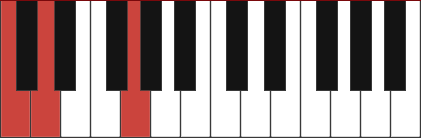
\includegraphics[width=0.2\textwidth]{assets/csus2.png}};
            \end{tikzpicture}} &
        \makecell[cc]{
            \chordscheme[
            ]} & \\
    \hline
    \makecell[cl]{
            Suspended} &
        \makecell[cl]{
            Csus4 } &
        \makecell[cl]{
            Perfect Fifth \\
            Perfect Forth \\
            Root} &
        \makecell[cc]{
            \raisebox{0ex}[5ex][1ex]{
                \musicintext{\staffbotmarg2\Interligne
                \Notes \zw{c}\zw{f}\qsk\zw{g}\en}}} &
        \makecell[cc]{
            \begin{tikzpicture}
                \node{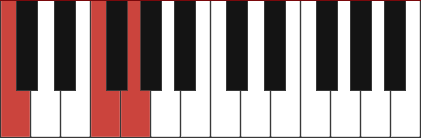
\includegraphics[width=0.2\textwidth]{assets/csus4.png}};
            \end{tikzpicture}} &
        \makecell[cc]{
            \chordscheme[
            ]} & \\
    \hline
\end{tabular}
}

\bigskip

\begin{center}
    \Large Other Info
\end{center}

\normalsize

"Slash" chords: the use of the slash in chord writing simply means that whatever is below the slash must be the bass note. Consequently, C/E indicates a C major triad with an E in the bass (first inversion). Be aware that there need not be a harmonic relationship between the chord above the slash and the note below it. This makes it possible to write chords that would be impossible to analyze in Roman numerals such as Cm/F$\sharp$.

A special situation arises when a minor seventh chord is placed in first inversion (for example: Am\textsuperscript{7}/C). While this notation will agree with traditional Roman numeral analysis, it will only rarely appear in jazz chord symbols. This type of chord would almost always be written as C\textsuperscript{6}; that is, a C major chord, with an added 6\textsuperscript{th} scale degree.

In Jazz, most chords are voiced with four pitches (regardless of the chord) and are played in the left hand near middle C. This sometimes means leaving out pitches and sometimes means adding pitches (triads are rare in jazz). See a chord glossary for specifics. The right hand would either play the tune, play a solo, or emphasize roots and 5ths.

\end{document}